\documentclass[journal]{IEEEtran}
\usepackage{iftex}
\ifXeTeX
\usepackage{newunicodechar}
\newunicodechar{–}{--}
\newunicodechar{—}{---}
\fi
\usepackage[T1]{fontenc}
\usepackage{cite}
\usepackage{amsmath,amssymb,amsthm,booktabs,array,url,graphicx}
\usepackage[hidelinks]{hyperref}
\usepackage{microtype}
\newcommand{\FPR}{\operatorname{FPR}}
\newcommand{\BA}{\operatorname{BA}}
\newcommand{\ind}{\mathbf{1}}
\newcommand{\ton}{TON-IoT}
\newcommand{\cic}{CICIoT2023}
\newcommand{\nb}{N-BaIoT}
\newtheorem{theorem}{Theorem}
\newtheorem{proposition}[theorem]{Proposition}
\newtheorem{definition}[theorem]{Definition}
\newtheorem{corollary}{Corollary}
\hyphenation{data-set data-sets pre-pro-cess-ing}
\makeatletter
\newcommand{\tableinput}[1]{\@@input #1.tex }
\makeatother
% Automatically generated from independent raw-log recomputation.
\newcommand{\RFEnergy}{1206.787}
\newcommand{\RFFOne}{0.983864}
\newcommand{\RFRecallPct}{99.664}
\newcommand{\RFFPRPct}{1.538}
\newcommand{\RFFN}{57.8}
\newcommand{\RFFP}{504.5}
\newcommand{\RFBatchMS}{32.595}
\newcommand{\TQEnergy}{1193.719}
\newcommand{\TQFOne}{0.970439}
\newcommand{\TQRecallPct}{96.710}
\newcommand{\TQFPRPct}{1.364}
\newcommand{\TQFN}{565.9}
\newcommand{\TQFP}{447.5}
\newcommand{\TQBatchMS}{1.447}
\newcommand{\TQSavingJ}{13.068}
\newcommand{\TQSavingJLow}{9.736}
\newcommand{\TQSavingJHigh}{16.400}
\newcommand{\TQSavingPct}{1.082}
\newcommand{\TQFOneDropPP}{1.343}
\newcommand{\TQRecallDropPP}{2.954}
\newcommand{\DQEnergy}{1200.560}
\newcommand{\DQFOne}{0.970439}
\newcommand{\DQRecallPct}{96.710}
\newcommand{\DQFPRPct}{1.364}
\newcommand{\DQFN}{565.9}
\newcommand{\DQFP}{447.5}
\newcommand{\DQBatchMS}{1.482}
\newcommand{\DQSavingJ}{6.227}
\newcommand{\DQSavingJLow}{1.600}
\newcommand{\DQSavingJHigh}{10.853}
\newcommand{\DQSavingPct}{0.515}
\newcommand{\DQFOneDropPP}{1.343}
\newcommand{\DQRecallDropPP}{2.954}
\newcommand{\CFEnergy}{1196.842}
\newcommand{\CFFOne}{0.636440}
\newcommand{\CFRecallPct}{99.335}
\newcommand{\CFFPRPct}{59.164}
\newcommand{\CFFN}{114.4}
\newcommand{\CFFP}{19405.9}
\newcommand{\CFBatchMS}{2.337}
\newcommand{\CFSavingJ}{9.945}
\newcommand{\CFSavingJLow}{7.117}
\newcommand{\CFSavingJHigh}{12.773}
\newcommand{\CFSavingPct}{0.824}
\newcommand{\CFFOneDropPP}{34.742}
\newcommand{\CFRecallDropPP}{0.329}

\begin{document}
\title{When Learned IDS Model Selection Collapses to a Static Choice: A Measurement Study at the Edge}
\author{Nuonan~Ouyang,
        Adrian~Shatte,
        Zhigang~Lu,
        Chao~Chen,~\IEEEmembership{Member,~IEEE,}
        and~Wei~Xiang,~\IEEEmembership{Senior Member,~IEEE}%
\thanks{(\textit{Corresponding author: Nuonan Ouyang.})}%
\thanks{N. Ouyang and A. Shatte are with the College of Science and Engineering, Division of Research, James Cook University, Bebegu Yumba Campus, Building 17, Douglas, Townsville, QLD, Australia (e-mail: nuonan.ouyang@my.jcu.edu.au; adrian.shatte@jcu.edu.au; ORCID: 0009-0004-7124-8940; 0000-0002-6225-9697).}%
\thanks{Z. Lu is with the School of Computer, Data and Mathematical Sciences, Western Sydney University, Penrith (Kingswood) Campus, Kingswood, NSW, Australia (e-mail: z.lu@westernsydney.edu.au; ORCID: 0000-0001-5102-6217).}%
\thanks{C. Chen is with the College of Business and Law, RMIT University, Melbourne, VIC 3000, Australia (e-mail: chao.chen@rmit.edu.au; ORCID: 0000-0003-1355-3870).}%
\thanks{W. Xiang is with the Australian Centre for AI in Medical Innovation and the Cisco-La Trobe Centre for AI and Internet of Things, La Trobe University, Melbourne, VIC, Australia (e-mail: w.xiang@latrobe.edu.au; ORCID: 0000-0002-0608-065X).}%
}
\markboth{IEEE Transactions on Network and Service Management,~Vol.~XX, No.~XX, Month~Year}%
{Ouyang \MakeLowercase{\textit{et al.}}: When Learned IDS Model Selection Collapses to a Static Choice}
\maketitle
\begin{abstract}
Runtime model selection trades detection quality against energy and latency. However, comparing a selector only with a more costly static detector conflates detector choice with the benefit of adaptation. We present a framework for analysis and physical measurement combining a pairwise reward criterion, matched static controls, paired blocks, a fixed load--prevalence factorial, and state-support reporting. On one Raspberry Pi 4B with four frozen TON-IoT detectors, tabular Q-learning and DQN both select LightLR throughout. A retrospective validation-only audit does not establish global LightLR optimality. In the corrected variable-load experiment, DeadlineGuard remains on MedRF and all methods record zero deadline misses. DQN and Q have energy differences of +0.60 J and +0.25 J against Static-LightLR, with paired 95\% intervals spanning zero; neither savings nor equivalence is established. Cascade saves 12.06 J against Static-MedRF at a 0.0446-percentage-point F1 cost, with lower recall and lower false-positive rate. These single-board results motivate joint audits of immediate reward preferences, realized actions, matched-static attribution, service feasibility and training support.

\end{abstract}
\begin{IEEEkeywords}
Intrusion detection, IoT, edge resource management, model selection, reinforcement learning, service management, energy measurement, reproducibility.
\end{IEEEkeywords}
\section{Introduction}
Edge intrusion detection systems (IDSs) must balance security, latency and energy on tightly constrained hardware~\cite{Zhang2024VehicleEdge,Murti2024vRAN,Zhang2024DVFO}. Runtime model selection may help, but a learned controller may simply select the same low-cost detector throughout. Comparing it only with a more costly static detector then credits adaptation with what is really a change of operating point. Reward normalization can cause this before training starts, by making preference reversals unattainable. Sparse coverage of discrete states can also hide an unsafe default action until the workload moves outside the training support. 

We address these risks with an analysis and measurement framework. First, a pairwise non-degeneracy criterion tests whether two actions exchange immediate-utility rank under the declared reward, fixed resource differences and validation support; it does not prove a long-horizon policy result. Second, the measurement protocol includes five components: trace-matched physical blocks, a static control using the detector selected by the policy, a factorial fixed before execution, joint raw/drift-adjusted reporting, and action reporting within and outside training support. Third, we apply the framework on one Raspberry Pi 4B with four frozen TON-IoT detectors, evaluating Tabular-Q, DQN, a fixed confidence cascade and DeadlineGuard. In the corrected variable-load comparison, Q and DQN remain LightLR and DeadlineGuard remains MedRF, reproducing the corresponding static controls' detection summaries. All methods have zero recorded deadline misses. Cascade uses 12.06 J less per 500-s run than Static-MedRF (paired 95\% CI $[-16.55,-7.58]$ J for Cascade minus MedRF), at a 0.0446-pp F1 cost. Historical fixed-load results remain separate, not pooled with these ten blocks.

The study addresses four research questions. \textbf{RQ1}: What security and resource operating points characterize the frozen detector pool? \textbf{RQ2}: Do learned selectors outperform the static schedule they realize, and does their reward allow preference reversals? \textbf{RQ3}: Do confidence- and deadline-aware controls provide useful switching under fixed and variable load? \textbf{RQ4}: How do state coverage, deadline violations, and threshold calibration using validation data only constrain deployment claims? We contribute a reproducible service-management method that distinguishes detector choice, conditional adaptation, objective design, and safety outside training support. We do not propose a new reinforcement learning (RL) algorithm. Fig.~\ref{fig:experimentdesign} shows the physical apparatus.

The remainder of the paper is organized as follows. Section~\ref{sec:relwork} reviews related work, and Section~\ref{sec:system} defines the system model and service objectives. Sections~\ref{sec:data}--\ref{sec:eval} describe the data, the detector pool, reward, and non-degeneracy criterion, and the evaluation protocol. Sections~\ref{sec:staticresults} and~\ref{sec:dynamicresults} report static/attribution and dynamic results, Section~\ref{sec:discuss} discusses implications, and Sections~\ref{sec:limits} and~\ref{sec:conclude} state limitations and conclude.

\begin{figure}[t]
\centering
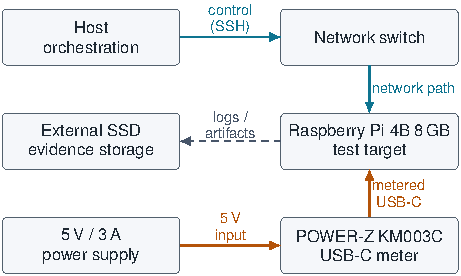
\includegraphics{figures/experiment_setup_schematic.pdf}
\caption{Physical apparatus. A 5-V supply feeds the Raspberry Pi 4B through the POWER-Z KM003C USB-C meter; host orchestration reaches the Pi through the network switch; the external SSD stores evidence artifacts. Teal: network/control; amber: power measurement; dashed: evidence storage. The drawing shows roles and paths only.}
\label{fig:experimentdesign}
\end{figure}

\section{Related Work}
\label{sec:relwork}
This work draws on edge IDS, conditional inference, model serving, and learned resource orchestration. Recent IDS research addresses continual detection, heterogeneous representations, and runtime model selection~\cite{Wang2024BFSNID,AOCIDS2024,StatAvg2025,DMIDS2025}. Auto-IDaS and FEDMS show that learned or confidence-driven detector selection is operationally plausible~\cite{Lin2024AutoIDaS,Hasan2026FEDMS}. However, neither controller complexity nor a lower-cost operating point alone establishes the value of adaptation. We therefore compare each selector with the static detector it actually uses and report the full state–action map alongside the occupancy of visited states.

Conditional-computation systems such as BranchyNet, adaptive network selection, MSDNet, and shallow–deep networks escalate uncertain inputs to costlier models~\cite{Teerapittayanon2016BranchyNet,Bolukbasi2017Adaptive,Huang2018MSDNet,Kaya2019ShallowDeep}. Our fixed confidence cascade applies this approach to whole-device IDS measurement. It also reveals a cost that row-level escalation rates can obscure. Only 1.34\% of rows are escalated, but these rows activate MedRF in 66.76\% of windows. Thus, call granularity, rather than the row fraction alone, governs the observed cost.

Serving systems such as Clipper, INFaaS, and Clockwork explicitly define service-level objectives (SLOs) for accuracy, latency, and cost, and route requests among model variants~\cite{Crankshaw2017Clipper,Romero2021INFaaS,Gujarati2020Clockwork}. We adopt this service-contract perspective and add two controls missing from these systems: a matched static action to separate the value of routing from model choice, and a pre-deployment audit to determine whether the declared reward allows preference reversals on validation support.

RL-based edge orchestration includes virtualized RAN (vRAN) reconfiguration, vehicle--edge scheduling, dynamic voltage and frequency scaling (DVFS), offloading, and QoS control~\cite{Murti2024vRAN,Zhang2024VehicleEdge,Zhang2024DVFO,Lou2024Startup,Kim2024DistributedOffload,Maleki2024QCS,Nan2026RobustDNN,Wang2025TrustOffload,Hu2025SITOff}. Tabular Q-learning and DQN are representative discrete and neural value-based controllers~\cite{Watkins1992,Mnih2015}. Our contribution to this line of work is a diagnostic methodology combining an analytic reward test, matched physical comparisons, a load–prevalence factorial design fixed before execution with an explicit deadline SLO, and an audit of actions outside training support. These components address known weaknesses in the evaluation of security ML and small-sample RL studies~\cite{Arp2022,Agarwal2021}.

\section{System Model and Service Objectives}
\label{sec:system}
An edge node processes batches in decision windows $t=1,2,\ldots$ using a resident detector pool $\mathcal M=\{m_1,\ldots,m_K\}$. Before inference, a frozen controller commits one action $a_t=\pi(s_t)\in\mathcal M$ from the causal state
\begin{equation}\label{eq:state}
s_t=(\widetilde T_t,h_{t-1},q_t,\lambda_{t-1},a_{t-1}),
\end{equation}
where $\widetilde T_t$ is smoothed temperature, $h_{t-1}$ the preceding selected detector's mean posterior, $q_t$ queue utilization, $\lambda_{t-1}$ preceding arrival count, and $a_{t-1}$ preceding action. This is the original fixed-load state; its 324-state policies, checkpoint rules and learning curves remain specific to that campaign. Corrected variable-load R2 instead uses $s_t^{\rm R2}=(N_t,Q_t^-,h_{t-1},a_{t-1})$, with current scheduled arrivals $N_t$ and raw FIFO carryover $Q_t^-$ measured before adding current arrivals (Section~\ref{sec:methods}). Ground truth, unselected current outputs, and cell identity are unavailable before action commitment. Cascade observes current-row LightLR confidence only after entry inference; that additional within-path information is not a predecision RL feature. All models remain resident, excluding fitting and loading cost.

For each completed window we record attack-class F1, recall, and false-positive rate; completion latency is checked against deadline $\Delta_{\rm SLO}$; and resource cost is whole-device USB energy. In the physical study $\Delta_{\rm SLO}=1$~s and each run lasts 500~s. Training optimizes a scalar surrogate, but evaluation jointly reports security, timeliness, energy, action occupancy, and state support. Test policies are frozen and never updated online.

The network-layer adversary may vary traffic prevalence and arrival rate but cannot alter the meter, controller memory, detector artifacts, or training pipeline. Adversarial-ML attacks and hardware tampering are outside scope. The operational risk considered here is induced entry into unvisited discrete states: deterministic ties can then expose an unaudited default action.

We credit a selector with \emph{adaptive value} only when it realizes more than one action on deployment support, improves a service objective without a comparable regression, and survives a paired comparison with the static instance of its dominant realized action. Otherwise the measured difference is attributed to detector operating-point choice rather than conditional adaptation.

\section{Dataset-Native Data Preparation}
\label{sec:data}
\subsection{Choice of Primary Dataset}
The primary systems study uses TON-IoT~\cite{Moustafa2021TONIoT,TONSource}. Its records combine IoT service telemetry, operating-system events, and networked interactions labeled with attack categories, making the dataset representative of the mixed-signal traffic that reaches an edge IDS at the service boundary rather than at the wire only. We deliberately restrict the physical dynamic-power study to a single dataset because coupling multiple encoded pipelines to one hardware campaign would confound feature dimensionality, class balance, and physical measurement; instead \cic{}~\cite{Neto2023CICIoT2023,CICSource} and \nb{}~\cite{Meidan2018NBaIoT,NBaIoTSource} are retained as supplementary detector and coverage audits and are not used to imply cross-dataset dynamic-power generalization.

\subsection{Frozen Preprocessing and Splits}
The TON-IoT pipeline is frozen and retains 32 native features. Imputation, scaling, and categorical encoding are fitted on training data only and applied deterministically to validation and test. The split groups unordered IP pairs so that traffic patterns are not divided across partitions; the grouping rule hashes ``$11\vert$'' concatenated with the sorted IP pair and thresholds the first sixteen SHA-256 hexadecimal digits modulo 100 (training below 60, validation 60--79, test 80--99). Training seed 11 fixes all model fits, so any single-seed conclusion is explicit rather than implied. Source-row identifiers and raw-field-string fingerprints are cross-partition disjoint, and an independent encoded-float32 audit finds \emph{zero} TON-IoT train--test vector matches, which addresses a commonly cited leakage risk in IoT IDS benchmarks~\cite{Arp2022}.

\subsection{Auxiliary Dataset Audits}
The same ledger retains dataset-native \cic{} and \nb{} pipelines with 39 and 115 native features respectively. For \cic{}, seventeen attack labels remain training-only because their capture files are too few for a defensible test split; the actual test taxonomy is a binary attack-versus-normal partition over sixteen attack categories plus benign traffic. For \nb{}, physical device identifiers are the grouping unit, giving five training, two validation, and two test devices; a post-hoc byte-level audit records that 17.3\% of \nb{} test rows share exact float32 vectors with training rows (seven distinct vectors), reflecting the sensor-repetition structure of the dataset rather than a preprocessing fault. These coverage and encoded-overlap limitations are retained rather than used to imply cross-dataset dynamic-power generality; consequently the auxiliary datasets support only static classification and replay evidence.

\subsection{Class Balance and Replay Traces}
Class balance differs by dataset. Attacks are a minority of the TON-IoT test split (5{,}361 of 22{,}490 rows, 23.8\%) but a large majority of the \cic{} and \nb{} test splits (94.6\% and 89.8\%). We do not rebalance, because the physical study measures whole-device behavior on the natural distribution; prevalence dependence is instead made explicit through~\eqref{eq:prevalence} and joint reporting of F1, recall, and FPR. To probe operating points under controlled prevalence shifts, the supplement retains fifty static replay traces: ten stationary traces per dataset and ten prevalence-shift traces each for TON-IoT and \cic{}, whose successive phase attack fractions are $\{0.05, 0.35, 0.70, 0.40, 0.10\}$ over $\{100, 100, 120, 100, 80\}$ windows. Each trace is evaluated with all four detectors (200 model--trace evaluations). These traces do not constitute a new detector-training exercise; they resample fixed held-out pools to expose how a frozen detector's F1 and balanced accuracy behave when class prevalence changes while each class's feature distribution is held fixed.

\section{Detector Pool, Reward Specification, and Non-degeneracy Framework}
\label{sec:methods}
This section specifies the frozen detector artifacts, the reward specification used by both learned controllers, and the pre-deployment pairwise non-degeneracy screening test. The last of these is stated as a theorem so that it can be applied to future learned selectors without re-derivation.

\subsection{Detector Pool}
Each dataset has four separately fitted configurations: depth-6 TinyDT; L2-regularized LightLR; 25-tree, depth-10 MedRF; and a 64/32/16 HeavyMLP. All use threshold 0.5 and training seed 11. Detector names do not assert a resource ranking; the physical measurements determine the empirical order. During TON-IoT physical experiments all models remain resident, and an action selects one model for the next batch without loading, fitting, or updating it. This design deliberately isolates the effect of controller decisions from model instantiation cost so that any observed switching cost is attributable to inference itself, not to hot-swapping detectors.

\subsection{Causal State Encoding}
In the original fixed-load setting, before window $t$ the controller constructs $s_t$ per~\eqref{eq:state}. The kernel temperature is smoothed as $\widetilde T_t=0.9\widetilde T_{t-1}+0.1T_t$, initialized at $T_0$. The threat observation $h_{t-1}$ is the arithmetic mean attack probability from the single detector selected in the preceding window; it is \emph{not} the preceding ground-truth attack fraction. Queue utilization is bounded to $[0,1]$, and the preceding arrival count is divided by 100 and bounded to $[0,2]$. Initial values are $h_0=0.5$, $\lambda_0/100=1$, and $a_0=\text{TinyDT}$.

Each of the first four state variables has three bins. Their two boundaries are $(45,70)$~$^{\circ}$C, $(1/3,0.7)$ for threat, $(1/3,2/3)$ for queue utilization, and $(0.9,1.1)$ for arrival ratio. Including four previous actions yields $3^4\times 4=324$ encoded states. Boundary equality enters the higher bin. The flat index is row-major in the listed order, with previous action changing fastest.

Corrected R2 instead encodes current arrivals $N_t$, raw FIFO carryover $Q_t^-$ before adding current arrivals, prior selected-path threat, and prior action. Arrival bins are $N_t\leq50$, $50<N_t\leq100$, and $N_t>100$; carryover bins are zero, 1--100, and above 100; threat bins are below $1/3$, $[1/3,0.7)$, and at least $0.7$. Prior action varies fastest, giving $3^3\times4=108$ states in arrival/carryover/threat/action order. Initial threat is 0.5 and prior action TinyDT. Temperature is safety-only; selected-path probabilities update threat after service.

The executed order within a window is: (i) state construction from causal telemetry and lagged context; (ii) action commitment and log; (iii) selected-detector inference; (iv) outcome log; and (v) lagged-state update for $t+1$. The information boundary of Section~\ref{sec:system} therefore holds at every decision; ground truth enters only offline training rewards, after the outcome is logged. This boundary is what allows preference-reversal analysis to be conducted purely on state features that the deployment can observe.

\subsection{Reward and Cost Provenance}
For the original fixed-load experiments, the unchanged per-window training reward is
\begin{equation}\label{eq:reward}
    r_t = 0.5\,B_t \;-\; 0.2\,\overline P_t \;-\; 0.2\,\overline L_t \;-\; 0.1\,\overline H_t,
\end{equation}
where $B_t$ is balanced accuracy over the classes present in the window. With $[x]_0^1=\min(1,\max(0,x))$, the normalization is
\begin{align}
    \overline P_t &= \biggl[\frac{P_t-2.347219336}{0.049806200}\biggr]_0^1,\\
    \overline L_t &= \biggl[\frac{L_t-1.2979595}{29.6547998}\biggr]_0^1,\\
    \overline H_t &= \biggl[\frac{\max(0,T_t^{\rm post}-\widetilde T_t)}{1\,^{\circ}\mathrm{C}}\biggr]_0^1.
\end{align}
$P_t$ and $L_t$ are frozen TON-IoT paced-profile lookups, not contemporaneous training measurements. Their means (power; batch latency) are 2.353132~W and 1.297960~ms for TinyDT, 2.347219~W and 1.544420~ms for LightLR, 2.397026~W and 30.952759~ms for MedRF, and 2.366688~W and 4.417836~ms for HeavyMLP. The compact software traces contain no post-action temperature response: their adapter supplies a fixed 35$^{\circ}$C predecision value and reuses that action-invariant value in the outcome field. Thus $\overline H_t=0$ throughout the executed training and validation traces; it is not an action-level thermal cost. No fitted thermal response or switching-energy penalty is used, and consequently no thermal control action is claimed.

Corrected R2 uses a separately frozen objective:
\begin{align}\label{eq:r2reward}
r_t^{\rm R2}={}&0.5 B_t-0.2\overline P_{a_t}-0.2\min(c_t,1)\nonumber\\
&-\ind[c_t>1\ \mathrm{or}\ Q_{t+1}>0]-\frac{Q_{t+1}}{N_t+Q_t^-},
\end{align}
with zero pending fraction for zero work. Training completion $c_t$ is $\lceil(N_t+Q_t^-)/100\rceil$ times the new warm-input p95 batch latency, in seconds. Power remains the historical TON min--max proxy, not contemporaneous variable-load energy. No thermal term is used. The fixed simulator develops no carryover, so queue ablation is not identifiable and is not executed; physical FIFO backlog is measured, not forced to zero.

\subsection{Pairwise Non-degeneracy Criterion}
Reward normalization is often reported as a hyperparameter without evidence that it permits any state to reverse the preferred action. We now show that this question can be answered before deployment with only the declared weights, cost profile, and a support region.

Consider two actions $a,b\in\mathcal M$. Decompose the scalar utility into a detection contribution and a normalized resource cost:
\begin{equation}
    U_a(s) = w_D\, D_a(s) - C_a,\qquad C_a=\sum_j w_j\,\overline C_{j,a},
\end{equation}
where $w_D=0.5$ in our specification and $\overline C_{j,a}$ collects the normalized resource penalties that are fixed on the declared support (as they are for the executed paced profiles at neutral thermal cost). Let $\Delta D_{ab}(s)=D_a(s)-D_b(s)$, $\Delta C_{ab}=C_a-C_b$, and $\tau_{ab}=\Delta C_{ab}/w_D$. Then
\begin{equation}\label{eq:diff}
    U_a(s)-U_b(s) = w_D\bigl(\Delta D_{ab}(s)-\tau_{ab}\bigr).
\end{equation}

\begin{theorem}[Pairwise non-degeneracy]\label{thm:nondeg}
Let $\mathcal S$ be a support region. Under the frozen scalar utility~\eqref{eq:diff}, a strict pairwise preference reversal between actions $a$ and $b$ exists on $\mathcal S$ if and only if
\begin{equation}\label{eq:nondeg}
    \min_{s\in\mathcal S}\Delta D_{ab}(s) < \tau_{ab} < \max_{s\in\mathcal S}\Delta D_{ab}(s).
\end{equation}
If \eqref{eq:nondeg} fails, the immediate difference cannot be strictly positive at one state and negative at another on $\mathcal S$. Thus an immediate-utility maximizer cannot reverse the pair there. This does not constrain a long-horizon RL policy when continuation values differ.
\end{theorem}

\begin{corollary}[Attainability under bounded detection]\label{cor:bound}
If $D_a(s),D_b(s)\in[0,1]$ for every $s\in\mathcal S$, then reversal is impossible whenever $|\tau_{ab}|\ge 1$; and reversal is guaranteed impossible whenever the attainable interval $[\min\Delta D_{ab},\max\Delta D_{ab}]$ does not straddle $\tau_{ab}$.
\end{corollary}

Because balanced accuracy lies in $[0,1]$, the corollary gives an immediate ceiling. Under the executed candidate-range scaling, the frozen nonthermal penalties imply $\tau_{\text{MedRF},\text{LightLR}}=0.7967$. A reproducible audit of all 2{,}500 windows in the five hash-bound validation traces finds $\Delta D_{\text{MedRF},\text{LightLR}}\in[-0.1053,0.1053]$, so this threshold lies outside the observed validation-window support. This retrospective audit excludes MedRF/LightLR and HeavyMLP/LightLR reversal on observed validation support. TinyDT/LightLR can reverse: TinyDT has higher immediate reward in 7 of 2{,}500 validation windows. These label-informed window comparisons establish neither optimality over all encoded states nor optimal long-horizon return, and do not fully explain the learned collapse. There is no evidence that this audit preceded test inspection. Supplementary Theorem~S1 gives the proof, Supplementary Table~S11A gives the full pairwise matrix, and Supplementary Algorithm~S1 gives the validation-only reward audit. If reversal is unattainable, the engineer should use an audited static schedule or renormalize against an external deployment contract---for example idle-relative power, the latency SLO, an energy envelope, or thermal headroom---rather than against detector-pool extrema.

The value $\tau\simeq0.7967$ belongs to the original fixed-cost reward only. Corrected R2 has load-dependent completion and service penalties, so this number is not transferred to its objective. Neither the theorem nor the corollary proves inevitable static RL behavior.

\subsection{Policies}
Four policy families are evaluated in the primary physical campaign. \emph{Static-\{TinyDT, LightLR, MedRF, HeavyMLP\}} freeze a single detector. \emph{CFSM} is a fixed heuristic initialized to TinyDT; at a smoothed temperature of at least 70~$^{\circ}$C it steps down one model rank, bypassing cooldown; otherwise it holds for two windows after a switch and steps down/up one rank when threat crosses 0.7. Queue and load are logged but not used by CFSM. \emph{Tabular-Q} uses zero initialization, $\alpha=0.1$, $\gamma=0.9$, and the update
\begin{equation}
    \begin{aligned}
        Q(s_t,a_t) &\leftarrow Q(s_t,a_t) + 0.1\,\delta_t,\\
        \delta_t &= r_t + 0.9\max_a Q(s_{t+1},a) - Q(s_t,a_t),
    \end{aligned}
\end{equation}
with zero terminal bootstrap~\cite{Watkins1992}. \emph{DQN} uses one-hot state, two 64-unit ReLU layers, Adam $10^{-3}$, replay 10{,}000, batch 32, and a target copy every 250 updates~\cite{Mnih2015}. In the original fixed-load setting both learners train for 1{,}000 episodes with $\varepsilon$ linearly annealed from 1 to 0.01; checkpoints are selected every 25 episodes on five validation traces. Test execution freezes the policy and performs no update.

Corrected R2 trains 25 artifacts using seeds 2003, 2011, 2017, 2027 and 2029: Q full/minus-arrival/minus-threat/minus-previous-action, and full-state DQN. Original learning hyperparameters are retained, but every run fixes its last checkpoint after 1,000 episodes of 500 windows. Full-state seed selection maximizes summed validation reward, ties choosing the lowest seed: Q 2011 and DQN 2003. The ten original training and five validation trace seeds are retained; validation resamples its existing pool. Historical test results were already viewed before this follow-up design. No physical result changes selection. Original checkpoint curves and training-time estimates do not describe these new runs.

Two causal policies are added in the R1/R2 campaigns (Section~\ref{sec:eval}). \emph{ConfidenceCascade} executes LightLR first and invokes MedRF on rows whose posterior lies in $[0.3,0.7]$; R1 uses 100-row windows, while corrected R2 serves FIFO batches of at most 100 rows. This post-entry confidence is not available to RL before window action commitment. In corrected R2, \emph{DeadlineGuard} selects MedRF when $\lceil(N_t+Q_t^-)/100\rceil L_{95}^{\rm RF}\leq1$~s and LightLR otherwise, using the same current arrivals and pre-append carryover exposed to RL. Its fixed calibration is not retuned using physical outcomes.

Archived process-start and policy-creation timestamps indicate approximately 26.7~s for the Tabular-Q training run and 256.9~s for DQN; these are provenance-derived wall-clock intervals rather than calibrated compute benchmarks, and training energy was not instrumented. Deployment cost is measured separately in Section~\ref{sec:dynamicresults}.

\section{Evaluation Protocol and Measurement Instrumentation}
\label{sec:eval}
Our evaluation protocol is designed to separate detector choice from adaptive value along five instruments: (i) paired physical blocks across trace-matched detectors; (ii) matched-static-action attribution controls; (iii) prospectively frozen factorial workloads; (iv) separate raw and drift-adjusted power endpoints; and (v) full occupancy and off-support action reporting. This section describes each instrument together with the classification, timing, and power measurement pipelines that feed them.

\subsection{Classification and Static Evidence}
The held-out classification evaluation uses the frozen threshold 0.5 and reports attack-class F1, recall, balanced accuracy, false-positive rate, and the full confusion counts. In particular,
\begin{align}
    \FPR &= \frac{FP}{TN+FP},\qquad F1 = \frac{2TP}{2TP+FP+FN},\\
    \BA &= \tfrac12\!\left(\tfrac{TP}{TP+FN}+\tfrac{TN}{TN+FP}\right).
\end{align}
Counts are pooled over the declared evaluation unit before metrics are calculated. The supplement retains 50 static traces and 200 model--trace evaluations; these reuse fixed held-out pools and do not constitute fresh attacks, classifier retraining, or physical repeats.

\subsection{Pi Prediction Consistency and Inference Timing}
Pi parity checks cover 12 dataset--model combinations and 10{,}000 encoded rows each with \emph{zero} threshold-label disagreements against the training-host outputs. Tight-loop timing reports 100-row inference after warm-up and excludes encoding, transport, queueing, and controller cost; these boundaries are re-stated wherever a timing figure is used.

\subsection{Static Whole-Device Power}
The physical reference uses one Raspberry Pi 4B 8~GB and an inline POWER-Z KM003C USB-C meter. Fifteen valid 1{,}800-second segments comprise three repeats of instrumented idle and four TON-IoT detectors, all resident, at 100 pre-encoded rows/s. This is resource characterization, not another detection test.

The meter records nominally 1~Hz boundary samples, including raw ADC replies, signed current, voltage, and monotonic request/receive times. Under the recorded connector orientation, consumed power is $P_i=V_i(-I_i)$. Using the observed sampling times $\tau_i$, input energy is approximated by
\begin{equation}\label{eq:trap}
    E=\sum_{i=1}^{n-1}\frac{P_i+P_{i+1}}{2}(\tau_{i+1}-\tau_i),\qquad
    \bar P = \frac{E}{\tau_n-\tau_1}.
\end{equation}
No missing sample is filled. This is 1-Hz load-side USB energy, not calibrated wall-side measurement or a subsecond waveform.

\subsection{Statistical Units and Interval Reporting}
For an outcome $z$ observed over $n$ declared repetitions, the two-sided Student-$t$ interval is
\begin{equation}\label{eq:tci}
    \bar z\pm t_{0.975,\,n-1}\,\frac{s_z}{\sqrt n},
\end{equation}
using the sample SD~\cite{NISTMean}. Physical scheduler inference uses \emph{ten paired blocks}, never rows, windows, or meter frames. Raw energy is primary. Drift sensitivity subtracts each run's immediately preceding idle power; it is reported separately rather than substituted for raw measurement. In the original campaigns, exact $2^{10}$ sign-flip tests supply a non-parametric robustness diagnostic under sign-symmetry and exchangeability, and are reported alongside the classical interval when both directional stability and magnitude precision matter.

Corrected R2 retains A: all valid blocks ($n=10$), B: exclude recovered block 1 ($n=9$), and C: exclude both recovered blocks 1 and 5 ($n=8$), each under raw and preceding-idle-adjusted endpoints. Exclusions were registered during execution at their actual times; all-pair enumeration was specified later. These are not retroactive original preregistrations. All nominal Student-$t$ intervals are retained without multiplicity correction or favourable selection; no equivalence margin was declared.

\subsection{Physical Campaigns Overview}
Six campaigns follow the static characterization; four of them (primary, P1A, R1, and R2) are metered whole-device campaigns. The \emph{primary} campaign contains ten matched 500-second blocks of Static-MedRF, CFSM, Tabular-Q, and DQN. \emph{P1A} adds ten matched blocks with Static-LightLR to enable the attribution comparison against the static action the learned policies realize. \emph{P1B} isolates state-to-action decision timing on the Pi. \emph{P1C--P1E} are software retraining studies of seed, reward/state, and Tabular-Q $\alpha/\gamma$ variations. \emph{R1} adds ten matched blocks at 100 rows/s comparing Static-LightLR, the confidence cascade, frozen Tabular-Q, and Static-MedRF. Corrected \emph{R2} uses separately frozen 108-state policies in ten matched blocks and six methods over the fixed $50/100/4000\text{ rows/s}\times 0.10/0.50/0.90$ prevalence factorial with a fixed one-second service deadline. Two additional protocols are recorded: \emph{R3} was predeclared for controller-only power measurement but stopped before execution because its four-state design condition became ambiguous once the frozen artifact was inspected; \emph{R4} is a post-hoc TinyDT threshold diagnostic conducted on validation only. R3 and R4 are reported in full because omitting either would misrepresent the executed evaluation surface. It is not pooled with historical variable-load execution, which had mismatched arrival visibility and post-append queue encoding.

\section{Static and Attribution Results}
\label{sec:staticresults}
This section reports the classification operating points, the static physical resource characterization, and the primary/P1A attribution and robustness evidence. Together these anchor the pairwise non-degeneracy analysis of Section~\ref{sec:methods} in measured, rather than declared, cost profiles.

\subsection{TON-IoT Detection Operating Points}
Table~\ref{tab:classification} shows the four TON-IoT operating points used by the physical study. TinyDT has recall 0.9976 but F1 0.4792 and FPR 67.78\%; LightLR, MedRF, and HeavyMLP have F1 0.9620--0.9746 and FPR 1.35--1.52\%. MedRF's aggregate held-out balanced-accuracy advantage over LightLR is 0.0140; this post-freeze test statistic is descriptive and is not treated as a statewise attainability bound. The non-degeneracy conclusion instead uses the validation-only window audit in Section~\ref{sec:methods}, where the observed difference range $[-0.1053,0.1053]$ does not straddle $\tau_{\text{MedRF,LightLR}}=0.7967$. Full confusion counts, plus \cic{}/\nb{} detector and overlap audits, are retained in the supplement.

\begin{table}[t]
\centering\footnotesize
\caption{TON-IoT held-out detection at threshold 0.5. BA denotes balanced accuracy; FPR is a percentage.}
\label{tab:classification}
\setlength{\tabcolsep}{4.2pt}
\begin{tabular}{lrrrr}\toprule
Model & F1 & Recall & BA & FPR (\%)\\\midrule
\tableinput{tables/ton_classification_rows}
\bottomrule\end{tabular}
\end{table}

For attack prevalence $p$, recall $r$, and FPR $f$,
\begin{equation}\label{eq:prevalence}
    F1 = \frac{2pr}{p(1+r) + (1-p)f},
\end{equation}
so high attack prevalence can coexist with high F1 and poor normal-class behavior. This identity motivates our decision to report attack-class F1, recall, and FPR jointly throughout, rather than summarizing with F1 alone.

\subsection{Static Physical Resource Measurements}
Across fifteen static segments, idle averages 2.335~W and active means span 2.347~W (LightLR) to 2.397~W (MedRF). MedRF's paired increment is 61.6~mW with 95\% CI $[32.1,\,91.0]$; TinyDT and LightLR intervals cross zero, indicating that the whole-device signal at this cadence is dominated by background platform power. No accepted workload window records undervoltage or throttling. Full segment statistics are supplementary; labels such as ``Tiny'' or ``Heavy'' are not used as empirical cost ranks.

\subsection{Primary Dynamic Comparison}
All forty primary runs contain 501 power samples and 500 decisions. Relative to Static-MedRF, Tabular-Q saves \TQSavingJ{} J (95\% paired CI \TQSavingJLow{}--\TQSavingJHigh{}) and DQN saves \DQSavingJ{} J (\DQSavingJLow{}--\DQSavingJHigh{}), but both lose \TQFOneDropPP{}~pp of F1 and \TQRecallDropPP{}~pp of recall. Both select LightLR in all 5{,}000 windows; consequently the primary contrast measures a detector operating-point change and not adaptive switching. This is the core observation that motivates the P1A attribution control below.

\subsection{P1A: Matched Attribution Against Static-LightLR}
P1A executes ten matched blocks comparing Tabular-Q, DQN, Static-LightLR, and Static-MedRF on the same traces. Because both learned policies realize LightLR throughout, Static-LightLR is the correct baseline for isolating adaptive value. Table~\ref{tab:p1a} reports three key paired contrasts.

\begin{table}[t]
\centering\footnotesize
\caption{P1A paired contrasts over ten trace-matched blocks. Each difference is first-minus-second method; intervals are Student-$t$ 95\% CIs, and $p$ is the exact two-sided sign-flip diagnostic over the ten block-level differences.}
\label{tab:p1a}
\setlength{\tabcolsep}{2.6pt}
\begin{tabular}{@{}lrrr@{}}\toprule
Outcome & Mean & 95\% CI & $p$\\\midrule
\multicolumn{4}{l}{\emph{Tabular-Q $-$ Static-LightLR}}\\
\hspace{0.4em}Energy (J)  & $+0.456$  & $[-1.861,\,+2.772]$   & 0.664\\
\hspace{0.4em}Power (mW)  & $+0.910$  & $[-3.722,\,+5.542]$   & 0.668\\
\multicolumn{4}{l}{\emph{DQN $-$ Static-LightLR}}\\
\hspace{0.4em}Energy (J)  & $+4.525$  & $[+2.693,\,+6.357]$   & 0.00195\\
\hspace{0.4em}Power (mW)  & $+9.045$  & $[+5.381,\,+12.709]$  & 0.00195\\
\multicolumn{4}{l}{\emph{Static-MedRF $-$ Static-LightLR}}\\
\hspace{0.4em}Energy (J)  & $+12.471$ & $[+10.611,\,+14.331]$ & 0.00195\\
\hspace{0.4em}F1 (pp)     & $+1.343$  & $[+1.292,\,+1.393]$   & 0.00195\\
\bottomrule\end{tabular}
\end{table}

Three findings emerge. First, Tabular-Q's energy contrast against the matched Static-LightLR control has an interval that includes zero, so the primary campaign's 13.1-J saving against Static-MedRF is fully explained by detector operating-point choice rather than by adaptation. Second, DQN carries a small but resolvable +4.5-J energy premium over Static-LightLR despite reproducing identical detection, indicating that its per-window controller cost, although a tiny fraction of each one-second window, is not free at 100 rows/s. Third, Static-MedRF's +12.5-J energy penalty against Static-LightLR is closely matched by the primary Tabular-Q saving against Static-MedRF, which confirms the compositional picture: (Static-MedRF $-$ Static-LightLR) $\approx$ (Static-MedRF $-$ Tabular-Q).

\subsection{P1B: Isolated Scheduler Overhead}
The isolated benchmark reports state-to-action decision time on the observed state support after correction of an earlier benchmarking substitution that was retained as an invalid attempt in the archive. On observed support, means are 0.739~$\mu$s for Static-LightLR, 6.582~$\mu$s for CFSM, 10.796~$\mu$s for Tabular-Q, and 1.567~ms for DQN. DQN is roughly $145\times$ Tabular-Q's controller cost but remains 0.157\% of the one-second decision interval. These timings are not converted into joules; the R2 physical evidence in Section~\ref{sec:dynamicresults} bounds what can be attributed to controller cost alone.

The full 240-unit benchmark, confidence intervals, and raw timing arrays are retained in Supplementary Table~S15.

\subsection{P1C--P1E: Multi-seed and Sensitivity Coverage}
P1C trains ten additional Tabular-Q and ten additional DQN policies under the frozen state, reward, split, and training-horizon protocol. All twenty policies select LightLR in 100\% of held-out windows (10/10 per algorithm; per-algorithm Wilson 95\% interval $[0.7225, 1.0]$). Greedy full-state maps vary across seeds---for DQN especially, from 0/324 to 311/324 TinyDT cells---but the observed-support behavior is unanimous, evidence for policy stability that is scoped to that support rather than to the whole encoded grid.

P1D varies reward weights and separately ablates state components; all 85 valid policies are single-action on held-out support. Only the five \emph{detection-only} Tabular-Q variants choose MedRF rather than LightLR, describing those runs rather than proving a necessary policy outcome. All thirty state-ablation policies remain LightLR. Fifteen minus-temperature, minus-queue and minus-arrival runs remove coordinates that never vary in training; they cannot establish adaptation to changes in those variables or identify them as irrelevant. Other ablations remain support-limited. P1E retains 35 Tabular-Q runs (five per setting) in one-at-a-time sweeps over $\gamma\in\{0,0.5,0.9,0.99\}$ and $\alpha\in\{0.05,0.10,0.20\}$; all thirty-five select LightLR.

The full P1C--P1E matrices are retained in Supplementary Tables~S16--S18. Together with Table~\ref{tab:p1a}, they document the observed collapse through matched attribution, isolated timing, and sanctioned reward/state/hyperparameter perturbations. Only removing all resource penalties changes the collapsed detector in this matrix; this is not a proof of global optimality.

\section{Dynamic Scheduler Results Under Fixed and Variable Load}
\label{sec:dynamicresults}
% Double-column floats are defined here so that they appear on the page where R1/R2 are discussed
% (LaTeX keeps single- and double-column floats in sequence).
\begin{table*}[t]
\centering\footnotesize
\caption{R1 fixed-rate physical results; means over ten paired blocks. Adjusted power subtracts the immediately preceding idle. Escalation is the fraction sent from LightLR to MedRF.}
\label{tab:r1}
\setlength{\tabcolsep}{4.0pt}
\begin{tabular}{lrrrrrrr}\toprule
Method & Energy (J) & Power (W) & Adjusted (mW) & F1 & Recall (\%) & FPR (\%) & Escalation (\%)\\\midrule
\tableinput{tables/r1_revision_rows}
\bottomrule\end{tabular}
\end{table*}

\begin{table*}[t]
\centering\footnotesize
\caption{Corrected R2 over ten paired blocks. Energy is mean$\pm$SD across runs; miss is the fraction of one-second windows missing deadline. Completion p95 is the mean of within-run 95th-percentile window completion times.}
\label{tab:r2}
\setlength{\tabcolsep}{3.1pt}
\begin{tabular}{lrrrrrrr}\toprule
Method & Energy (J) & Power (W) & F1 & Recall (\%) & FPR (\%) & Miss (\%) & Completion p95 (s)\\\midrule
\tableinput{tables/r2_revision_rows}
\bottomrule\end{tabular}
\end{table*}

\begin{figure*}[!t]
\centering
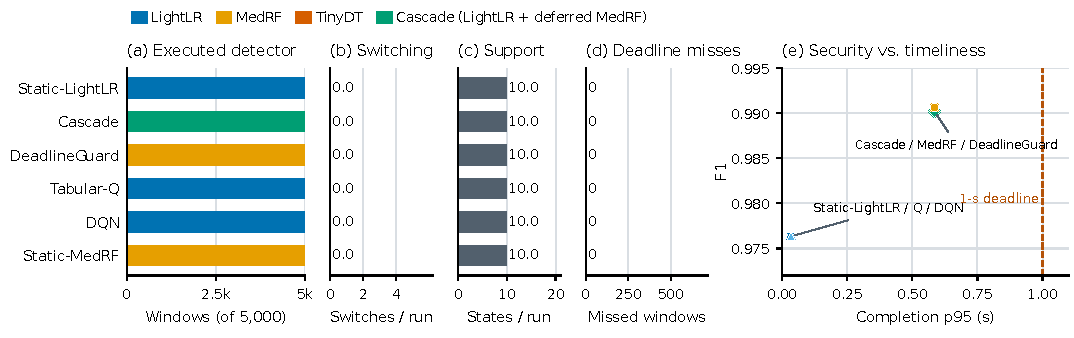
\includegraphics[width=\textwidth]{figures/r2_operational_dashboard.pdf}
\caption{Corrected R2 operational summary across 60 runs: (a) executed paths; (b) runtime action changes, excluding initialization; (c) unique 108-state indices per run; (d) deadline misses; (e) F1 versus mean run-level completion p95, with the 1-s deadline dashed. Q/DQN stay LightLR, DeadlineGuard stays MedRF, and all methods have zero recorded misses. Cascade denotes a conditional LightLR-plus-MedRF path, not a single-detector action.}
\label{fig:r2dashboard}
\end{figure*}

This section retains the fixed-rate R1 campaign and reports the corrected variable-load R2 comparison separately from historical variable-load execution. R1 uses its original fixed-load policies; corrected R2 uses the 108-state service-penalized setting in Section~\ref{sec:methods}. R3 remains a protocol-preserving stop and R4 a validation-only threshold diagnostic. No historical and corrected measurements are pooled.

\subsection{R1: Fixed-Rate Confidence Cascade}
Table~\ref{tab:r1} reports ten new matched blocks at 100 rows/s. The fixed cascade escalates 1.34\% of rows and raises F1 by 1.347~pp over Static-LightLR while spending +7.952~J with 95\% CI $[5.897,\,10.007]$~J. Its raw mean-power difference is +15.917~mW $[11.798,\,20.035]$, whereas the preceding-idle adjustment gives +13.635~mW $[-1.515,\,28.784]$: environmental drift therefore weakens the power attribution but not the raw-energy result. Cascade F1 (0.98391) matches Static-MedRF (0.98386) within a few $10^{-5}$, at 0.279~pp lower recall and 0.156~pp lower FPR.

\subsubsection*{Cascade cost is a call-granularity phenomenon, not a bound}
The apparently disproportionate cascade latency at a 1.34\% escalation rate is explained by call granularity. The frozen source performs \emph{one} MedRF call per escalation-active window on the deferred sub-batch, not one MedRF call per deferred row. Although only 1.3388\% of the 500{,}000 rows are deferred, they land in 3{,}338 of 5{,}000 windows (66.76\%), with a mean of only 2.01 deferred rows per active window. No-escalation windows average 1.636~ms; any-escalation windows average 31.884~ms, close to the cost of a single MedRF batch call regardless of sub-batch size; the overall mean is 21.830~ms. This is an operating-point description, not a general bound: an optimized batched cascade with wider windows or amortized MedRF calls would show a different profile. What the measurement establishes is that reporting only the escalation \emph{fraction} would be misleading; escalation \emph{prevalence across windows} is the operational cost driver.

\subsection{R2: Variable-Load Factorial and DeadlineGuard}
Each corrected R2 run visits the nine fixed load-by-prevalence cells for 50 windows each, followed by 50 recovery windows. All methods receive the same workload within block; no cell identity or label is an online feature. The learned controllers and DeadlineGuard share current arrivals and pre-append carryover; Cascade additionally observes current-row confidence after entry inference. Table~\ref{tab:r2} gives all six means and Table~\ref{tab:r2pairs} gives matched-static and cascade contrasts.

\begin{table}[t]
\centering\footnotesize
\caption{Headline R2 paired contrasts ($n=10$ blocks). Differences are first-minus-second method; F1 and deadline-miss changes are percentage points.}
\label{tab:r2pairs}
\setlength{\tabcolsep}{5pt}
\resizebox{\columnwidth}{!}{%
\begin{tabular}{lrrr}\toprule
 & Cascade $-$ & Q $-$ & DQN $-$\\
Endpoint & Static-MedRF & Static-LightLR & Static-LightLR\\\midrule
\tableinput{tables/r2_key_paired_rows}
\bottomrule\end{tabular}}
\end{table}

\subsubsection*{DeadlineGuard: no realized load-conditioned switching}
DeadlineGuard executes MedRF in all 5{,}000 windows, as does Static-MedRF; both have identical within-block detection summaries and zero recorded misses. Its calibrated demand test never triggers LightLR on these traces. Static-LightLR, Q, DQN and Cascade also record zero misses. Hence the corrected experiment does not demonstrate deadline-violation removal, load-triggered switching gains or a superiority claim for DeadlineGuard. The historical 43.7-J/512-miss result arose under a different execution interface and is not a corrected-R2 result.

Cascade minus Static-MedRF has mean energy difference $-12.064$~J, paired 95\% CI $[-16.548,-7.580]$~J. F1 changes by $-0.0004457$ ($-0.0446$~pp), recall by $-0.2411$~pp, and FPR by $-0.1534$~pp. Lower FPR thus accompanies lower recall and F1, not a cost-free improvement. This variable-load trade-off is implementation-specific; it is not the historical 1.373-pp DeadlineGuard comparison or the fixed-rate R1 call-cost regime.

\subsubsection*{Learned selectors and matched static controls}
Corrected Q and DQN each select LightLR in every one of their 5{,}000 windows and reproduce Static-LightLR detection exactly. Their mean energy differences from Static-LightLR are respectively +0.246~J $[-4.055,4.547]$~J and +0.599~J $[-4.119,5.317]$~J. Neither interval resolves an energy benefit; neither proves equivalence. The historical Tabular-Q TinyDT trajectory used mismatched load timing and post-append queue normalization and is retained as an implementation diagnostic, not evidence that the corrected common-interface policy fails on new load bins. The original 314/324 map remains specific to its original fixed-load policy.

\subsubsection*{Interrupted blocks and preceding-idle sensitivity}
Block 1 retains five accepted methods plus a newly numbered Static-LightLR replacement after external CPU rejection; block 5 retains its accepted runs and replaces the failed Cascade idle before its first formal workload. Both span periods. A maintenance task coincides with the first failure; the second revealed processing overhead added to a fixed sampling wait. The monitor repair changes wait cadence and rejected-gap logging, not the 5\% CPU or 1.5-s interval limits. The old rejected right snapshot is absent, so its exact gap cannot be reconstructed. We report all-valid A, exclude-block-1 B, and exclude-blocks-1/5 C under raw and idle-adjusted endpoints (Supplementary Table~S24). Registration timing is disclosed; no favourable set is selected. Idle adjustment does not establish removal of temporal or instrumentation confounding. Figure~\ref{fig:r2dashboard} reports the corrected occupancy, service and state observations. The old DQN block-4 excursion remains a separate historical diagnostic without precise CPU-joule attribution.

\subsection{R3: Protocol-Preserving Stop}
R3 predeclared controller-only physical power over four ``original observed-support states'' for isolated attribution. The frozen artifact exposes eight such states and supplies no outcome-independent rule for selecting four. Choosing four \emph{after the fact} would allow controller-power reporting to be driven by known R2 results, so the campaign stopped before measurement per the predeclared stop rule. No controller-only joule value is claimed. Its stop remains unchanged; neither the corrected DQN--LightLR contrast nor timing is assigned a controller-only joule interpretation.

\subsection{R4: Threshold Calibration Diagnostic}
R4 selects a TinyDT threshold on validation by maximum balanced accuracy (highest-threshold tie-break), hashes it, and applies it \emph{once} to test. Table~\ref{tab:r4} contrasts the frozen primary threshold with the validation-selected diagnostic.

\begin{table}[t]
\centering\footnotesize
\caption{TON-IoT TinyDT test results at the fixed primary threshold and the post-hoc validation-selected threshold. The diagnostic does not replace the primary threshold; it isolates calibration sensitivity as an explanation for the primary failure.}
\label{tab:r4}
\setlength{\tabcolsep}{5pt}
\begin{tabular}{lrr}\toprule
Quantity & Primary (fixed) & Validation-selected\\\midrule
\tableinput{tables/r4_threshold_main_rows}
\bottomrule\end{tabular}
\end{table}

The diagnostic yields F1 0.9698, FPR 1.82\%, recall 99.61\%, BA 0.9889, and AUROC 0.9906. Recall changes by only 0.15~pp, so the primary failure at threshold 0.5 is substantially calibration-sensitive rather than a symptom of missing ranking information. Two consequences follow. First, TinyDT is not rehabilitated for the frozen physical campaigns: every classifier and scheduler artifact in those campaigns was fixed at threshold 0.5, and no post-hoc threshold can retroactively undo the historical TinyDT actions emitted under the earlier R2 interface; corrected R2 does not select TinyDT. Second, calibration governance---validation-only threshold selection with a hashed freeze before test---is a deployable practice that we recommend for any operational IDS pipeline that includes a TinyDT-class detector.

\section{Discussion}
\label{sec:discuss}
\subsection{Attribution and Conditional Value}
The primary 13.1-J Tabular-Q saving against Static-MedRF is only 26.1~mW over 500~s, while false negatives rise almost tenfold (57.8 to 565.9 per run). P1A resolves no Tabular-Q difference against its realized Static-LightLR control; that historical result concerns detector choice rather than adaptation. Corrected R2 likewise resolves no Q/DQN benefit over Static-LightLR, while DeadlineGuard stays MedRF and all methods record no misses. The new Cascade--MedRF comparison instead combines lower energy with slightly lower F1/recall and lower FPR. In the separate fixed-rate R1 regime, 1.34\% deferred rows activate MedRF in 66.76\% of windows: call granularity, not row fraction alone, controls serving cost.

\subsection{External-Budget Normalization Rule}
Theorem~\ref{thm:nondeg} screens immediate pairwise preferences under fixed resource differences, not long-horizon policy optimality. For the original fixed-cost reward, candidate-range scaling yields $\tau_{\text{MedRF,LightLR}}=0.7967$, outside its observed validation range $[-0.1053,0.1053]$. It does not transfer to the corrected load-dependent completion/deadline/backlog reward. A portable design replaces pool extrema with external denominators:
\begin{align}
\overline P_a&=\frac{P_a-P_{\rm idle}}{B_P}, &
\overline L_a&=\frac{L_a}{\Delta_{\rm SLO}},\\
\overline E_a&=\frac{E_a}{B_E}, &
\overline H_a&=\frac{[T_a-T_{\rm safe}]_+}{B_T},
\end{align}
where $B_P$, $\Delta_{\rm SLO}$, $B_E$, and $B_T$ are operator-set power, latency, energy, and thermal budgets. These denominators remain interpretable when the detector pool changes. The validation-only audit should be run before policy freeze; if no relevant pair can reverse, use an audited static schedule or redesign the pre-test contract.

\subsection{Support, Safety, and Measurement}
The original fixed-load Tabular-Q maps 314/324 states to TinyDT because unseen zero-initialized rows tie and \texttt{np.argmax} chooses action zero. That remains a default-action warning, but historical R2's post-append queue and unequal arrival timing do not isolate algorithmic load generalization. Corrected R2 instead trains and deploys the shared 108-state semantics; its Q and DQN stay LightLR. Training carryover remains zero, so neither successful encoding nor the deletion of constant coordinates establishes queue-adaptation competence. Deployments should retain both action maps and actual training/deployment support.

Small whole-device effects require paired blocks and joint raw/drift-adjusted reporting. Corrected R2 retains both recovered-block exclusion sets as well; temporal recovery and monitor cadence remain possible confounders. The original DQN excursion lacked the later process-aware guard and supports no precise background-process or controller-power allocation. R3 supplies no controller-only power. The practical checklist remains: audit immediate reward attainability; include the realized static action and causal controls; fix load/threat schedules before execution; report confusion counts, deadlines, occupancy and support; retain all raw/adjusted sensitivities; and select detector thresholds on validation only.

The portable contribution is this audit-and-attribution framework, not a universal numeric ranking. Corrected R2's Cascade trade-off, the separate R1 call-granularity result and original controller timings are conditional on their own Pi, resident pool, batching and instrumentation settings; they are not interchangeable costs.

\section{Limitations and Reproducibility Boundary}
\label{sec:limits}
Classifier results use one training seed, fixed dataset-native splits, and threshold 0.5; replay reuses held-out pools. Only TON-IoT receives dynamic physical testing. Ten paired blocks on one Raspberry Pi 4B 8~GB do not estimate board, meter, site, or fleet variability, and CICIoT2023/N-BaIoT are not dynamic-power evidence.

The ChargerLAB POWER-Z KM003C (HW~2.4, FW~2.0.6) was not independently laboratory calibrated. Its nominal 1-Hz load-side USB measurements exclude AC conversion, packet capture, and feature encoding. Models remain resident, temperatures stay low, and the factorial is scheduled feature replay rather than live traffic. The software-policy traces contain only a constant 35$^{\circ}$C predecision fallback and no action-attributable post-action temperature; the executed thermal reward is therefore zero and cannot establish thermal-aware adaptation. Pairing cannot remove ambient drift; R3 supplies no controller-only joule value; and R1 cascade cost is specific to 100-row windows.

P1 controls and R4 are post-hoc to the primary campaign; R1 and the original R2 were fixed for their own execution. Corrected R2 was designed after historical test inspection; validation-only selection does not restore an unseen test. Blocks 1 and 5 span recovery periods; A/B/C sensitivities are actual campaign-time additions, not original preregistrations. The reward audit is retrospective, and cannot establish execution before test inspection. Its earlier implementation read aggregate test confusion counts for a descriptive diagnostic; the corrected entry point excludes those inputs. The corrected software adapter reports missing post-action temperature as null and flags the unavailable measurement; the thermal penalty is omitted rather than treated as a measured zero. Historical results are retained unchanged. The 15 constant-coordinate ablations do not validate adaptation; corrected training carryover is also constant. A predecision EMA is a state feature, not a measured action-caused temperature increment. No equivalence margin was declared. Invalid attempts and authorized replacements remain archived. No nominal paired interval establishes equivalence; multiplicity is not corrected. The theorem assumes a linear utility with $w_D>0$ and support-fixed normalized costs; non-linear objectives, switching penalties, and load-dependent costs require support-conditioned extensions.

\section{Conclusion}
\label{sec:conclude}
The pairwise non-degeneracy criterion tests immediate action-pair reversal under fixed resource differences, while matched-static attribution distinguishes adaptation from detector choice. The original fixed-load results and corrected variable-load experiment both show learned policies realizing LightLR on their measured support. Corrected R2 resolves no energy benefit against Static-LightLR and does not establish equivalence; DeadlineGuard remains MedRF and all methods have zero recorded misses. Cascade saves 12.06~J against Static-MedRF with a small F1/recall reduction and lower FPR, an implementation-specific trade-off. Learned orchestration should be credited only after objective assumptions, realized actions, matched controls, service feasibility, training support and whole-device measurement are audited together.

\bibliographystyle{IEEEtran}
\bibliography{references}
\end{document}
